\toptitle{[ELEC-H-201] Électricité et électronique}{TP3}
\TPtitle{Électricité et électronique\vspace*{2mm}}{TP3:\vspace*{2mm}
Réalisation d'un amplificateur audio - 2\up{e} partie: câblage et test du montage}

\frontpage{consignes3.tex}
\vspace{5cm}
\newpage

\section{Manipulation}
\subsection{Introduction}
Lors de ce laboratoire, vous allez câbler sur un protoboard l’amplificateur audio analysé au labo précédent (TP2: Réalisation d'un amplificateur audio - 1\up{ère} partie : analyse du montage). Pour réaliser un montage clair, il est important de respecter quelques règles qui vous sont données ci-dessous.
\subsubsection{Positionnement sur le protoboard}
Afin de pouvoir visualiser votre montage et ainsi retrouver les erreurs éventuelles, il faut regrouper le plus possible les composants d’un étage (= un bloc) dans une même zone et mettre les différents étages dans l’ordre du schéma.
\subsubsection{Code couleurs}
L’utilisation d’un code couleurs pour les fils qui relient vos composants permet de bien distinguer les fils servant pour les différentes alimentations et pour les signaux.
Pour faciliter la tâche des assistants, nous vous avons défini un code couleur (il n’existe pas un code standard, mais généralement, le noir est utilisé pour les fils de masse et le rouge pour l’alimentation) :

\begin{itemize}
\item Alimentation +12V : mauve
\item Alimentation +5V : rouge
\item Masse : noir
\item Alimentation -12V : bleu
\item Signaux : autres que ceux utilisé pour les alimentations
\end{itemize}

Les montages qui ne respectent pas ce code ne seront pas corrigés!

\subsubsection{Longueur des fils}
Tout conducteur (notamment tout fil) est une antenne qui peut capter les parasites environnants. Ces parasites proviennent de plusieurs sources telles que les néons, antennes GSM, … La quantité de parasites dépend de la longueur des fils: plus les fils utilisés sont longs, plus vous capterez de parasites. De plus, des fils longs nuisent à la clarté de votre montage.
Il est donc impératif d’utiliser des fils les plus courts possibles. Plusieurs pinces à dénuder et coupante seront à votre disposition dans le laboratoire.

\subsubsection{Vérification de chaque étage}
Il est toujours plus difficile de trouver les erreurs dans un gros montage que dans un plus petit. Il faut donc tester vos étages séparément. Après avoir réalisé un bloc et avant de le connecter au précédent, mettez à son entrée un signal (à l’aide du générateur) et mesurez le signal de sortie: est-il bien celui que vous attendez?

\subsection{Montage}
Nous allons réaliser ce montage étage par étage. Les schémas de branchement des composants intégrés sont donnés à la fin de ce document.
\subsubsection{Étage d’entrée}
Comme nous l’avons vu au premier labo, cet étage sert d’adaptation d’impédance et d’une première amplification.

\begin{itemize}
\item Câblez-le.
\item Ajoutez un signal d’entrée sinusoïdal variant entre -200mV et 200mV et de fréquence de 500Hz.
\item Visualisez les signaux d’entrée et de sortie à l’oscilloscope.
\item Vérifiez que le circuit réalise bien un gain de 40. Si ce n’est pas le cas, vérifiez votre montage et retestez-le.
\end{itemize}

\subsubsection{Filtre + volume des basses}
La première partie de ce bloc est un filtre passe-bas de fréquence de coupure de 595Hz et la seconde permet de régler le volume des basses.

\begin{itemize}
\item Câblez ce montage sans le raccorder au premier étage.
\item Ajoutez un signal d’entrée sinusoïdal variant entre -4V et 4V et de fréquence de 100Hz.
\item Visualisez les signaux d’entrée et de sortie à l’oscilloscope.
\item En bougeant le potentiomètre, vous devriez voir le signal de sortie varier.
\item Mettez le gain à 1 et augmentez la fréquence à 6kHz
\item Observez l’effet du filtre passe-bas.
\end{itemize}

\subsubsection{Filtre et volume des aigus}
Ce bloc est similaire au précédent à la différence du filtre qui est un passe-haut de même fréquence de coupure.

\begin{itemize}
\item Câblez ce montage sans le raccorder au premier étage.
\item Ajoutez un signal d’entrée sinusoïdal variant entre -4V et 4V et de fréquence de 2kHz.
\item Visualisez les signaux d’entrée et de sortie à l’oscilloscope.
\item En bougeant le potentiomètre, vous devriez voir le signal de sortie varier.
\item Mettez le gain à 1 et diminuez la fréquence à 50Hz
\item Observez l’effet du filtre passe-haut.
\end{itemize}

\subsubsection{Étage sommateur + volume}
Cet étage permet de mélanger les deux signaux provenant de l’étage précédent et de régler le volume.

\begin{itemize}
\item Câblez ce montage sans le raccorder à l’étage précédent.
\item Ajoutez un signal sinusoïdal variant entre -1V et 1V et de fréquence de 500Hz sur une des entrées. Branchez l’autre entrée sur l’alimentation 5V.
\item Visualisez les signaux d’entrée et de sortie à l’oscilloscope.
\item En bougeant le potentiomètre, vous devriez voir le signal de sortie varier.
\end{itemize}
\subsubsection{Assemblage}
\begin{itemize}
\item Raccordez tous vos étages déjà câblés.
\item Vérifiez à l’aide d’un signal d’entrée que votre circuit réalise toute les fonctions voulues.
\end{itemize}

\subsubsection{Étage de sortie}
Cet étage est un amplificateur de puissance spécialement conçu pour des applications audio de faible puissance sonore.

\begin{itemize}
\item Câblez ce montage sans le raccorder à l’étage sommateur.
\item Ajoutez un signal d’entrée sinusoïdal variant entre -2V et 2V et de fréquence 500Hz.
\item Observez VO1 sur le canal 1 de l’oscilloscope et VO2 sur le canal 2. Remarquez qu’ils ont la même composante continue et des composantes alternatives en opposition de phase.
\end{itemize}

\subsubsection{Test du montage complet}
\begin{itemize}
\item Raccordez l'amplificateur de puissance au reste de votre circuit.
\item Branchez le diviseur résistif, le câble jack et le haut-parleur à votre ampli.
\item Testez en le bon fonctionnement.
\item Félicitations: vous venez de fabriquer votre premier amplificateur audio !
\end{itemize}











\newpage
\section*{ANNEXE A: Schéma de montage}
\label{montagetotal}
\begin{minipage}{.7\textwidth}
\begin{center}
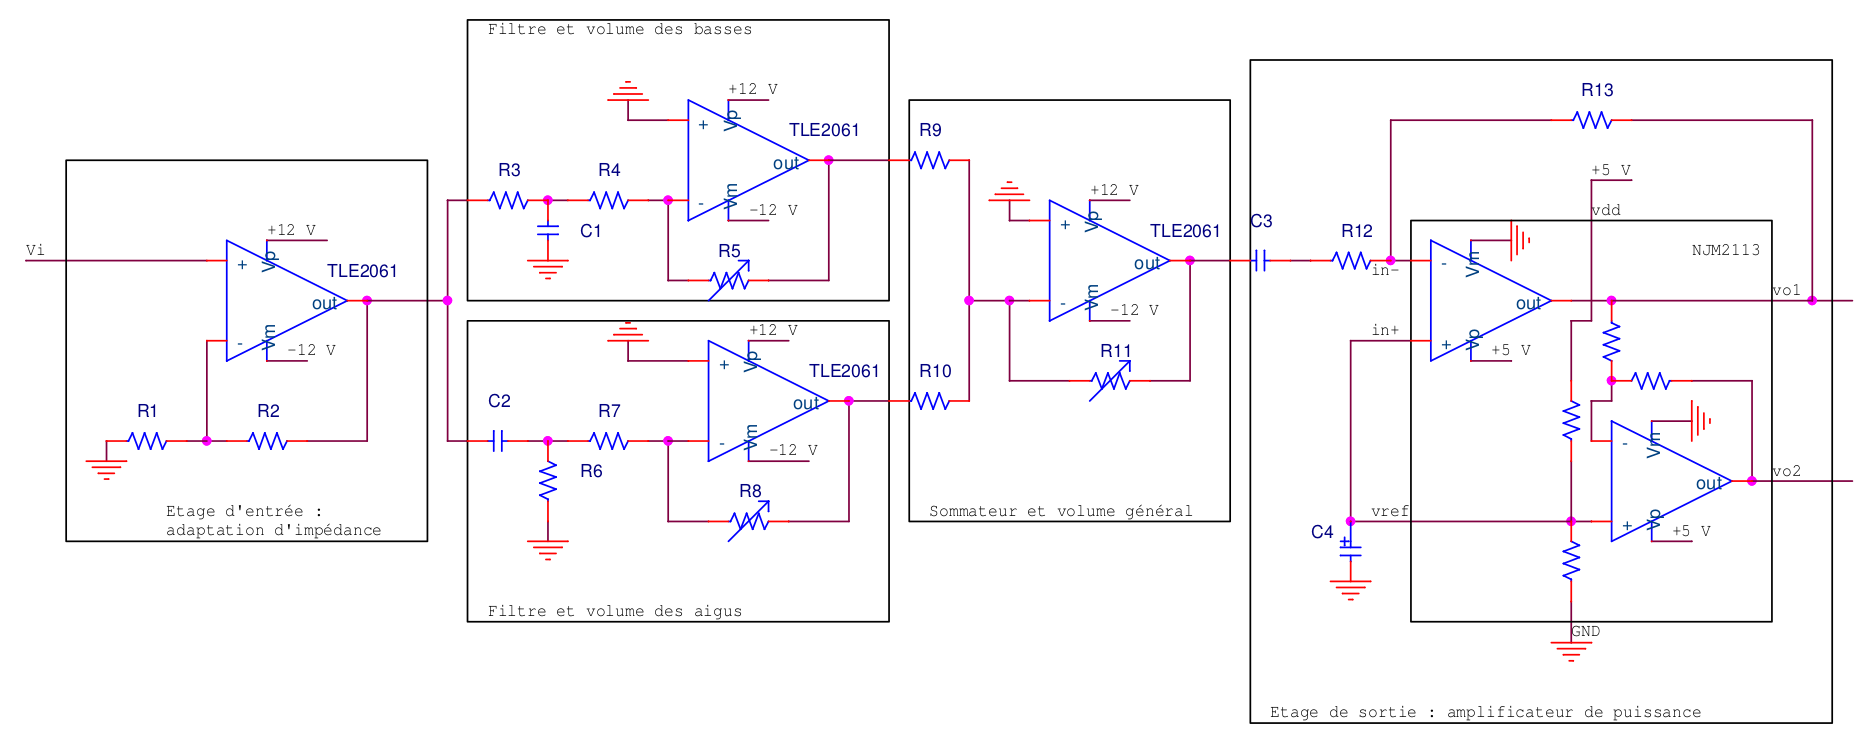
\includegraphics[width=23cm, angle=90]{decoupageenblocs.PNG}
\end{center}
\end{minipage}
\begin{minipage}{.25\textwidth}
\begin{center}
\rotatebox{90}{
\begin{tabular}{|c|c|c|c|c|c|}\hline
$R_1 = 1 k\Omega$ & $R_2 = 39 k\Omega$ & $R_3 = 2.7 k\Omega$ & $R_4 = 100 k\Omega$ & $R_5 = 100 k\Omega$ & $R_6 = 2.7 k\Omega$ \\ \hline
$R_7 = 100 k\Omega$ & $R_8 = 100 k\Omega$ & $R_9 = 22 k\Omega$ & $R_{10} = 22 k\Omega$ & $R_{11} = 100 k\Omega$ & $R_{12} = 22 k\Omega$ \\ \hline
$R_{13} = 22 k\Omega$ & $C_1 = 100 nF$ & $C_2 = 100 nF$ & $C_3 = 330 nF$ & $C_4 = 1 \mu F$ & \\ \hline
\end{tabular}
}
\end{center}
\end{minipage}


\section*{ANNEXE B: Datasheet TLE2061}
\vspace{-0.1cm}
\label{DatasheetTLE2061}
\begin{center}
\includegraphics[scale=0.8, page=2]{tle2061.pdf}
\end{center}

\section*{ANNEXE C: Datasheet NJM2113}
\vspace{-0.1cm}
\label{DatasheetNJM2113}
\begin{center}
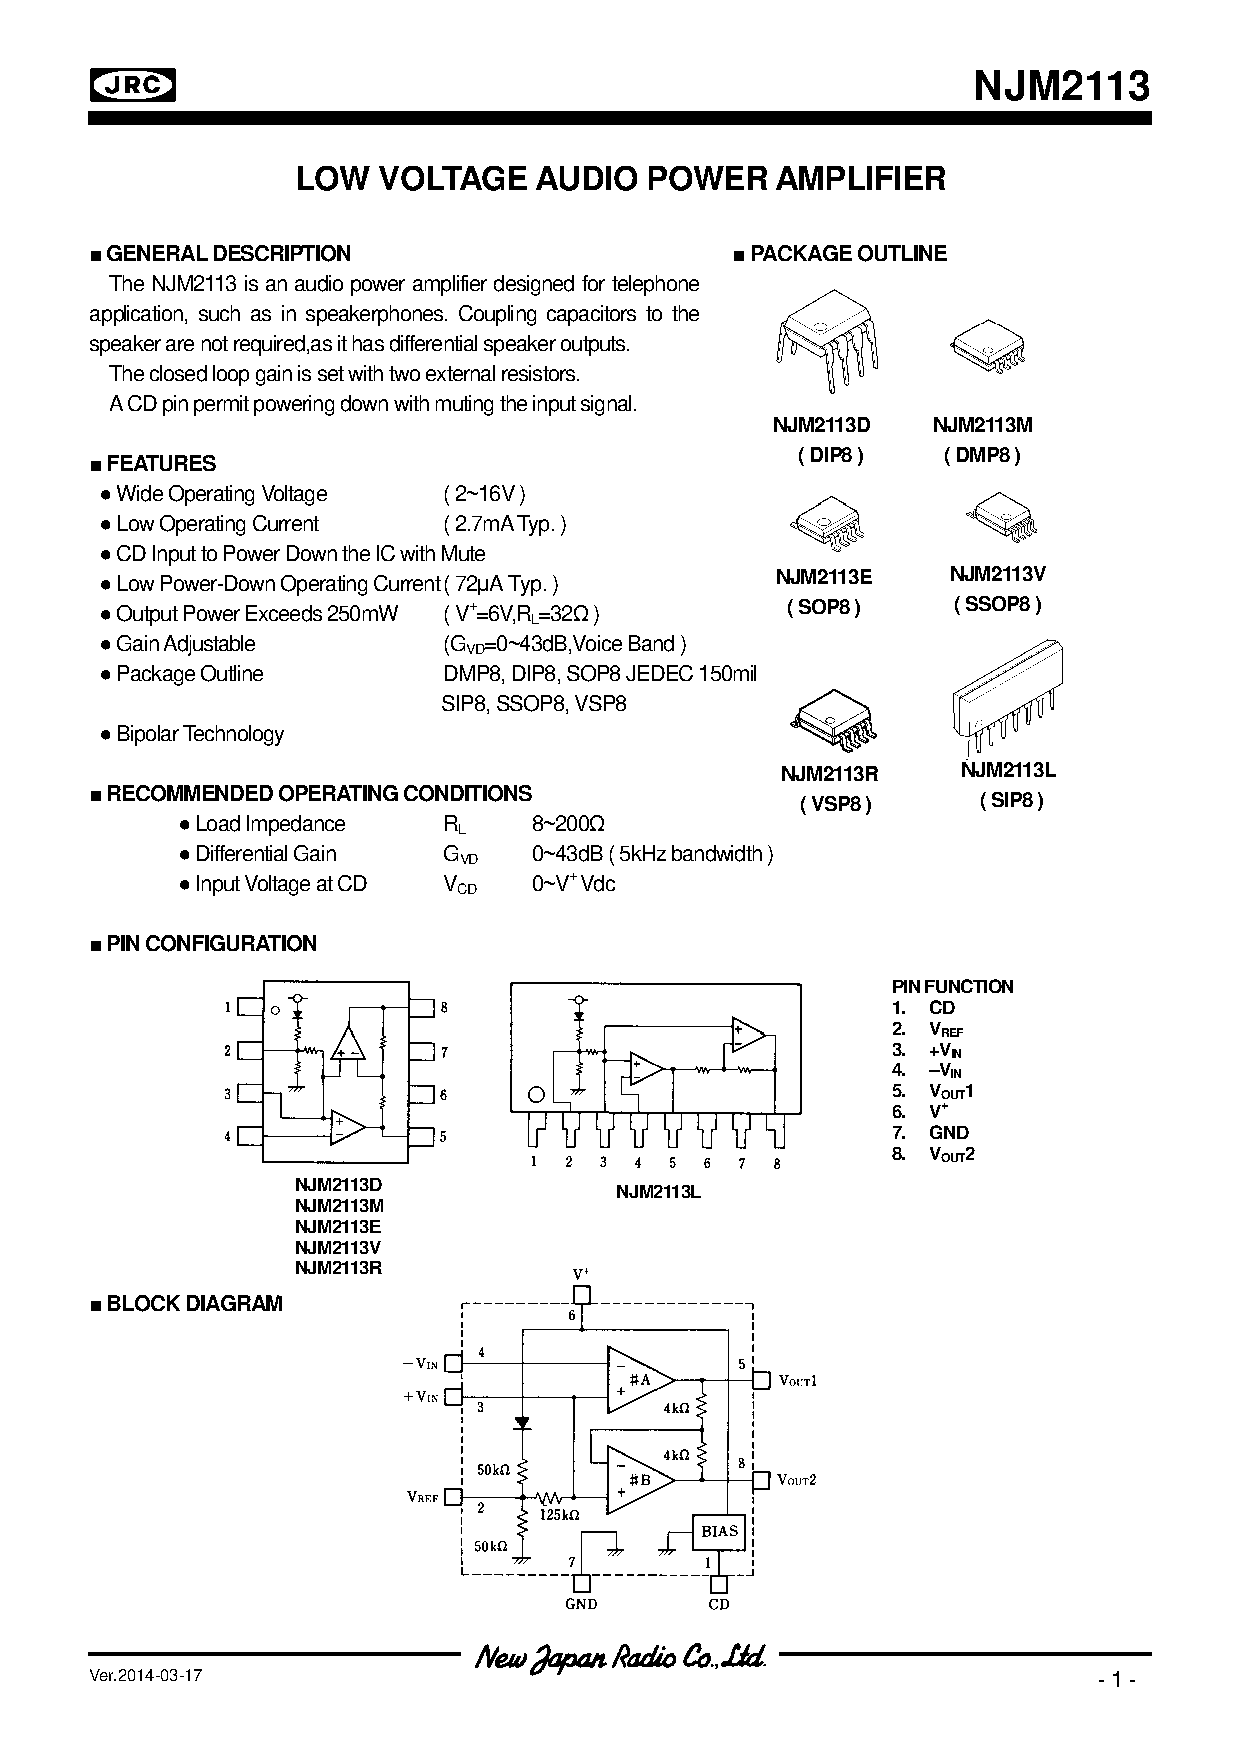
\includegraphics[scale=0.8, page=1]{NJM2113_E.pdf}
\newpage
\includegraphics[scale=0.9, page=3]{NJM2113_E.pdf}
\end{center}

\endinput
